%!TEX root = proposta.tex 
%% Matheus renomeia "exemplo.tex" para um nome mais descritivo (e muda a linha acima)
\chapter{\label{chap:conte}Contexto}

\todo[color=red,author=Felipe,inline]{Ok, aqui está bem genérico, agora começa a projetar parágrafo por parágrafo do material que tu já leste (bullets para cada parágrafo), e me manda depois que tu completares o texto. Deixa as bullets no topo para eu entender o teu raciocínio}

\section{Planejamento} 

Planejamento é o modo racional de agir. Planejamento é a geração de um plano para atingir um objetivo. O processo do planejamento consistem em escolher e gerenciar as ações, antecipando os resultados a fim de atingir um objetivo pré definido \cite{ghallab2004automated}. \\
Para que alguns objetivos consigam ser alcançados, as ações que são tomadas não necessariamente necessitam de um planejamento, nas atividades do dia-a-dia a maioria das ações que são tomadas não são planejadas. Para fazer um planejamento é avaliado os ganhos de planejar as ações em vista do objetivo, geralmente, os planos nem sempre são os melhores possíveis, pois a busca de planos considerados perfeitos são mais demorados para construir, fazendo com que planos razoáveis ou bons sejam escolhidos ao invés dos perfeitos \cite{ghallab2004automated}. \\
Pelo fato de se ter alguns tipos de ações, também há alguns formas de planejamento \cite{ghallab2004automated}. Algumas das formas de planejamento são:

\begin{itemize}
	\item Planejamento de trajetória e movimento - Este tipo de planejamento foca em problemas onde é preciso simplificar um caminho de um ponto inicial a um objetivo e ainda controlar a trajetória através do caminho. Por exemplo, gerar a rota de um caminhão e movimento de um braço mecânico. 
	\item Planejamento de percepção - Este tipo de planejamento é focado em problemas onde os planos devem se preocupar com as informações obtidas pelo sistema. Por exemplo,  a construção de um ambiente virtual de uma área urbana através de imagens. 
	\item Planejamento de navegação - Combina os dois tipos acima de planejamento, de percepção e movimento, para problemas que precisem da combinação de localizações e percepções. Por exemplo, andar por um rio desviando de obstáculos.  
\end{itemize}

Planejamento na computação é a área da Inteligencia Artificial(IA) que busca a geração de planos automaticamente de forma computacional \cite{ghallab2004automated}. E para representar o processo de planejamento no computador é preciso de um modelo conceitual que é um recurso teórico usado para descrever o problema de forma geral e assim podendo aprofundar dependendo da abordagem. Como planejamento é  focado na escolha de ações para acontecer mudança de estados no sistema, o modelo para descrever esse processo deve ser dinâmico, ou seja, que permita a mudança do ambiente\cite{ghallab2004automated}. \\

O modelo geral utilizado para representar um plano é o \textit{state-transition systems}. O modelo é representado por $\sum = (S, A, E, \gamma) $. Onde S representa os estados, A as ações, E os eventos que podem ocorrer no sistema, e $\gamma$ a função de transição composta por $ \gamma: S \times A \times E \rightarrow S'$. A figura \ref{fig:planmodelo} mostra uma representação desse modelo \cite{ghallab2004automated}.


\begin{figure}[ht]
	\centering
	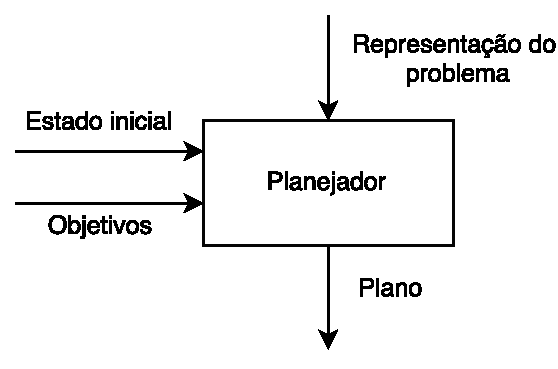
\includegraphics[width=0.4\textwidth]{fig/modelo.pdf}
	\caption{Modelo de estado e transição}
	\label{fig:planmodelo}
\end{figure} 

Um plano é gerado, quando dado um estado inicial e um objetivo, um conjunto de ações é gerado e quando executadas levam ao objetivo. O processo usado para conseguir isso é chamado de planejamento, onde é necessário ter uma descrição do sistema($\sum$) onde os estados e as ações são definidos.\\ 
Os estados são representados por um conjunto de átomos sem função \cite{intelligence2003modern}, que são usados para representar alguma situação, por exemplo uma pessoa estar em um lugar pode ser representado por \textit{at(Matheus, PUCRS)}, assim todos os estados devem seguir o padrão, podendo ter mais de uma situação, como por exemplo, representar que alguém está em um lugar e feliz ao mesmo tempo, \textit{at(Matheus,PUCRS) $\wedge$ happy(Matheus)}. \\
As ações são descritas por um conjunto esquema de ações \cite{intelligence2003modern}. Para toda ação é necessário uma pré condição aplicada ao estado atual, que se for satisfeita, garante o efeito ou pós condição, levando o sistema para o estado resultante. Por exemplo, caminhar de um lugar a outro: \\
\textit{Action(walk(from, to)): \\
Precond: at(from)  $\wedge$ path(from,to) \\
Effect: $\neg$ at(from)  $\wedge$ at(to)}

\subsection{HTN} 
Dentro do planejamento existe um tipo especifico chamado \textit{Hierarchical Task Network Planning} (HTN). Os métodos de HTN são utilzados pelo fato do problemas serem descrito como receitas, seguindo uma ordem de execução das tarefas, que pode corresponder como pessoas pensam em resolver problemas de planejamento \cite{ghallab2004automated}.  \\
A grande diferença de planejamento HTN dos demais tipos de planejamento é o fato de que as ações são tratadas em mais alto nível \cite{intelligence2003modern}. As ações vão sendo decompostas até serem diretamente executadas, um bom exemplo é viajar de avião, a tarefa principal é viajar de um lugar para o outro, mas antes disso deve-se comprar a passagem e ir até o aeroporto de táxi para então conseguir realizar a viagem. 

Em HTN as ações são chamadas de tarefas e a finalidade não é alcançar o objetivo, e sim realizar um conjunto de tarefas que resolvam um determinado problema. Como entrada para o sistema é necessário um conjunto de operadores e um conjunto de métodos. Em HTN as ações são chamadas de tarefas, e podem ser dividas em dois tipos: Primitivas e não primitivas. As tarefas primitivas são executadas diretamente através do conjunto de métodos, já as tarefas não primitivas são decompostas recursivamente em sub tarefas e assim se transformando em tarefas menores até se tornarem em tarefas primitivas, e assim podem ser executadas. A figura \ref{fig:travelmethods} mostra um exemplo de descrição dos métodos para uma viagem de avião.

\begin{figure}[ht]
	\centering
	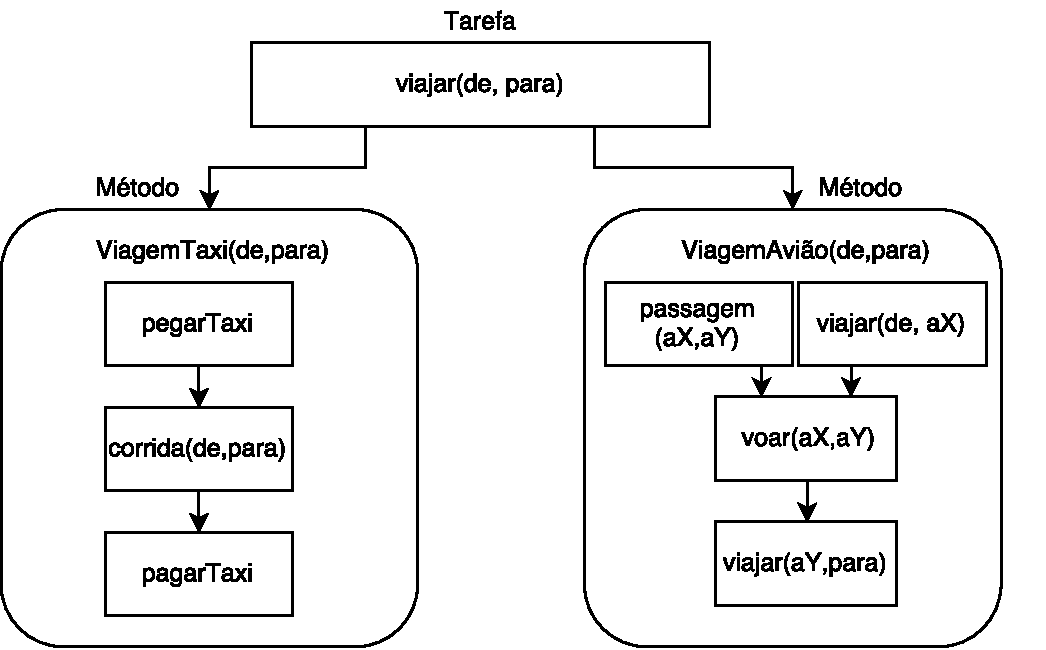
\includegraphics[width=0.8\textwidth]{fig/travelmethod.pdf}
	\caption{Exemplo de problema de HTN}
	\label{fig:travelmethods}
\end{figure}  

O planejamento HTN executa todas as possibilidades de resolução do problema, sempre respeitando a ordem dos métodos que conseguem ser realizados, quando um caminho de resolução leva a um fim de linha é realizado um retrocesso(\textit{backtracking}) até um caminho que tenha uma possibilidade de caminho diferente do que foi tomado anteriormente.

\subsection{AHTN} 

%AHTN é HTN + game tree search \cite{adversal}
\textit{Adversarial hierarchical-task network} (AHTN) é um algoritmo proposto para tentar solucionar o problema do grande fator de ramificação dos jogos em tempo real \cite{ontanon2015adversarial}. O algoritmo combina técnicas de planejamento HTN e o algoritmo \textit{minimax game tree search}. \\
%explicar Game search tree(minimax)
%explicar técnica de HTN utilizada
%explicar diferença do minimax puro

\subsection{Motivação e aplicação}
A motivação para o estudo de planejamento automatizado vem do fato que, como planejamento é um componente vital do comportamento racional, e a IA busca alcançar aspectos de inteligencia a nível computacional, então planejamento é um elemento chave para isso\cite{ghallab2004automated}.
%algumas aplicações de planejamento e exemplos

\section{Aprendizado} 
%-overview de aprendizado
%**O que é em geral \\
Para os humanos o aprendizado ocorre durante toda a vida. O aprendizado é o ato de adquirir novos conhecimentos, ou modificar conhecimentos já existentes ou ainda adquirir uma experiencia por repetição do ato de forma incorreta. Aprendizado pode variar de adquirir conhecimento de tarefas simples, como decorando um numero de telefone, até tarefas mais complicadas, como a formulação de novas teorias \cite{intelligence2003modern}. \\
Na computação o aprendizado depende de alguns fatores \cite{intelligence2003modern}:
\begin{itemize}
	\item Qual o conhecimento que será melhorado ou descoberto.
	\item Qual o conhecimento que o sistema já possui.
	\item Qual é a representação usada por esse conhecimento.
	\item Qual é o aprendizado disponível de fato.
\end{itemize}


\subsection{Aprendizado de Máquina} 

% o que é aprendizado de maquina
% Definição de ML: aprende atráves de um experiencia E em uma tarefa T com uma performace P  
% reinforcement o que é - aprendizado atráves de um conjunto de simulações
% explicar Q LEARNING

\subsection{Motivação e aplicação}
%motivação
%aplicação no mundo real com exemplos


%\section{Jogos Real-time Strategy(RTS)} 

%Jogos eletrônicos são muito populares, não só entre os jovens, principalmente pela grande quantidade de gêneros, existem jogos de ação, aventura, esportes, estrategia, entre outros. \\
%Dentro dos jogos de estratégia há uma subseção que se chama jogos de estratégia em tempo real, neles os jogadores estão se enfrentando no mesmo momento, como o nome já diz. Em alguns desses jogos há BOTs(jogadores que simulam um jogador real) e é preciso alguma inteligencia para esses BOTs conseguirem levar graça ao jogador real, para isso é utilizado algoritmos de IA. Esse tipo de jogo, devido a sua grande quantidade de ações, possui um fator de ramificação muito grande, e cresce exponencialmente, com isso aplicar os algoritmos se torna uma tarefa não trivial.  \\